% !TeX program = xelatex
\documentclass{article}
\usepackage{kotex}
\usepackage[a4paper,left=3cm, right=3cm, top=2cm, bottom=2cm]{geometry}
\usepackage{amsmath}
\usepackage{graphicx}
\usepackage{caption}
\usepackage{setspace}
\usepackage{xcolor}
\usepackage{titlesec}
\usepackage{amssymb}
\usepackage{tcolorbox}
\usepackage{wrapfig}
\usepackage{amsthm}
\usepackage{multirow} 
\usepackage{array}
\usepackage{tcolorbox}
\usepackage{pgfplots}
\pgfplotsset{compat=1.18}% For proofs

\graphicspath{{graph/}}
\title{7.1 곡면의 종류}
\date{}
\author{}
\setstretch{1.3}

% \subsection* 형식 지정 (번호 없음)
\titleformat{name=\section, numberless}
  {\normalfont\large\bfseries\color{blue}}
  {}
  {0pt}
  {}
\geometry{a4paper, margin=1in}

% 증명 환경 스타일
\newtheoremstyle{mystyle}% name
  {}% Space above
  {}% Space below
  {\itshape}% Body font
  {}% Indent amount
  {\bfseries}% Theorem head font
  {.}% Punctuation after theorem head
  {.5em}% Space after theorem head
  {}% Theorem head spec (can be left empty, meaning `normal')
\theoremstyle{mystyle}

\begin{document}
\maketitle

\begin{tcolorbox}[colback=blue!5, colframe=blue!60!black, title=7.1 곡면의 종류 -- 한눈에 보기, boxrule=0.5mm, arc=3mm]
\begin{center}
\renewcommand{\arraystretch}{1.3}
\begin{tabular}{|p{2.2cm}|p{5cm}|p{6.5cm}|}
\hline
\textbf{종류} & \textbf{생성 방법} & \textbf{판별 포인트} \\
\hline
구면 & 중심에서 일정 거리(반지름) & 표준형 $(x-a)^2+(y-b)^2+(z-c)^2=r^2$ \\
\hline
주면 & 도선(곡선) + 평행 이동 모선 & 한 변수가 방정식에 없다 \\
\hline
추면 & 도선 + 정점을 지나는 모선 & 동차방정식(원점이 정점) \\
\hline
회전면 & 평면곡선을 축에 대해 회전 & 두 변수를 $\sqrt{\square^2+\square^2}$로 치환 \\
\hline
\end{tabular}
\end{center}
\end{tcolorbox}

3차원 공간에서 방정식 \(f(x,y,z)=0\)을 만족시키는 점의 자취는 일반적으로 \textbf{곡면}, 두 방정식 \(f=0,\ g=0\)을 동시에 만족시키는 자취는 일반적으로 \textbf{곡선}이다.

\section*{[1] 구면 (Sphere)}

\begin{tcolorbox}[
    colback=teal!4,
    colframe=teal!65!black,
    title=정의 \& 핵심 규칙,
    fonttitle=\bfseries,
    boxrule=0.5mm,
    arc=3mm
    ]
    \textbf{\textcolor{teal!65!black}{정의.}}\quad
    중심 \(C(a,b,c)\), 반지름 \(r\)인 \textbf{구면}(sphere):
    \[
    (x-a)^2+(y-b)^2+(z-c)^2=r^2
    \]

    \noindent\textcolor{teal!50!black}{\rule{\linewidth}{0.4pt}}

    \textbf{\textcolor{teal!65!black}{핵심 규칙.}}\quad
    전개하면 \(x^2+y^2+z^2+2Ax+2By+2Cz+D=0\) 꼴이 되고, 다시 완전제곱으로 되돌리면
    \[
    (x+A)^2+(y+B)^2+(z+C)^2=\underbrace{A^2+B^2+C^2-D}_{R^2}
    \]
\end{tcolorbox}

% ---- 그림 삽입 위치 1: 구면 (중심-반지름 개념도) ----

\begin{center}
\renewcommand{\arraystretch}{1.3}
\begin{tabular}{|l|l|l|}
\hline
\(R^2\)의 부호 & 의미 & 중심/반지름 \\
\hline
\(R^2>0\) & 구면 & 중심 \((-A,-B,-C)\), 반지름 \(R\) \\
\hline
\(R^2=0\) & 점구 (점 하나) & \((-A,-B,-C)\) \\
\hline
\(R^2<0\) & 허구 (실수해 없음) & --- \\
\hline
\end{tabular}
\end{center}

\begin{figure}[h]
\centering
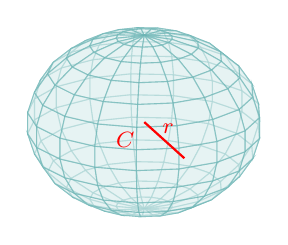
\begin{tikzpicture}
\begin{axis}[hide axis, view={115}{20}, width=5.5cm, height=5.5cm]
\addplot3[
    surf, shader=faceted, faceted color=teal!60, fill=teal!12, opacity=0.55,
    domain=0:180, domain y=0:360, samples=14, samples y=18, z buffer=sort,
]
({1.3*sin(x)*cos(y)}, {1.3*sin(x)*sin(y)}, {1.3*cos(x)});
\addplot3[thick, red] coordinates {(0,0,0) (0.92,0.92,0)};
\node at (axis cs:0,0,0)[anchor=north east, red]{\footnotesize $C$};
\node at (axis cs:0.55,0.55,0)[anchor=south, red]{\footnotesize $r$};
\end{axis}
\end{tikzpicture}
\caption{구면: 중심 $C$와 반지름 $r$}
\end{figure}

\subsection*{EXAMPLE 1 (아폴로니우스 구면)}
두 정점 \(O(0,0,0),\ Q(a,0,0)\ (a\ne0)\)로부터 거리의 비가 일정한 점 \(P(x,y,z)\)의 자취.\\
\textbf{SOLUTION:} \(OP:PQ=k:1\)에서 \(x^2+y^2+z^2=k^2\{(x-a)^2+y^2+z^2\}\), 즉
\[
(1-k^2)(x^2+y^2+z^2)+2ak^2x=k^2a^2
\]
\[
\Rightarrow\quad
\begin{cases}
k=1 & x=\dfrac{a}{2}\text{ 인 평면}\\[6pt]
k\ne1 & \left(x+\dfrac{ak^2}{1-k^2}\right)^2+y^2+z^2=\left(\dfrac{ak}{1-k^2}\right)^2 \text{ 인 구면}
\end{cases}
\]

\section*{[2] 주면 (Cylinder)}

\begin{tcolorbox}[
    colback=teal!4,
    colframe=teal!65!black,
    title=정의 \& 핵심 규칙,
    fonttitle=\bfseries,
    boxrule=0.5mm,
    arc=3mm
    ]
    \textbf{\textcolor{teal!65!black}{정의.}}\quad
    곡선(\textbf{도선})을 따라 평행하게 움직이는 직선(\textbf{모선})이 만드는 곡면이 \textbf{주면}(cylinder)이다.

    \noindent\textcolor{teal!50!black}{\rule{\linewidth}{0.4pt}}

    \textbf{\textcolor{teal!65!black}{핵심 규칙.}}\quad
    방정식에 한 변수가 없으면, 그 변수의 축에 \emph{평행한} 모선을 가진 주면이다.
    \begin{itemize}
        \item \(f(x,y)=0\) (z 없음) $\to$ \(xy\)평면에 수직인 주면
        \item \(f(z,x)=0\) (y 없음) $\to$ \(zx\)평면에 수직인 주면
        \item \(f(y,z)=0\) (x 없음) $\to$ \(yz\)평면에 수직인 주면
    \end{itemize}
\end{tcolorbox}

\begin{center}
\renewcommand{\arraystretch}{1.4}
\begin{tabular}{|l|l|}
\hline
방정식 & 이름 \\
\hline
\(x^2+y^2=r^2\), \((x-h)^2+(y-k)^2=r^2\) & 원주면 \\
\hline
\(\dfrac{x^2}{a^2}+\dfrac{y^2}{b^2}=1\), \(\dfrac{(x-h)^2}{a^2}+\dfrac{(y-k)^2}{b^2}=1\) & 타원주면 \\
\hline
\(\dfrac{x^2}{a^2}-\dfrac{y^2}{b^2}=1\), \(\dfrac{(x-h)^2}{a^2}-\dfrac{(y-k)^2}{b^2}=1\) & 쌍곡주면 \\
\hline
\(y^2=4px\), \((y-k)^2=4p(x-h)\) & 포물주면 \\
\hline
\end{tabular}
\end{center}

% ============ 이미지 삽입 위치: 주면 정의/핵심규칙 박스 직후 ============
% 도선(빨간 원, 밑면 곡선)을 따라 모선(파란 평행선)이 움직여 주면을 만드는 과정을 시각화.
\begin{figure}[h]
\centering
\begin{tikzpicture}
\begin{axis}[hide axis, view={115}{20}, width=6.5cm, height=6.5cm]
% 주면 몸체 (반투명 원기둥)
\addplot3[
    surf, shader=faceted, faceted color=teal!45, fill=teal!10, opacity=0.4,
    domain=0:360, domain y=0:2.6, samples=24, samples y=8, z buffer=sort,
]
({1.3*cos(x)}, {1.3*sin(x)}, {y});
% 도선 (밑면 곡선, 빨강 강조)
\addplot3[thick, red, domain=0:360, samples=40, samples y=0]
({1.3*cos(x)}, {1.3*sin(x)}, {0});
% 모선 (도선을 따라 평행하게 움직이는 직선들, 파랑)
\foreach \ang in {0,45,90,135,180,225,270,315}{
  \addplot3[thick, blue!70!black] coordinates
    {(1.3*cos(\ang),1.3*sin(\ang),0) (1.3*cos(\ang),1.3*sin(\ang),2.6)};
}
\node at (axis cs:1.3,0,2.9)[blue!70!black]{\footnotesize 모선};
\node at (axis cs:0,-1.3,-0.3)[red]{\footnotesize 도선};
\end{axis}
\end{tikzpicture}
\caption{주면: 도선(빨강)을 따라 모선(파랑)이 평행하게 움직이며 곡면을 만든다}
\end{figure}

\subsection*{EXAMPLE 2}
주면 \(x^2=4py\ (p>0)\)을 그려라.\\
\textbf{SOLUTION:} \(z=0\)일 때 방정식은 \(xy\)평면 위의 포물선(도선). 이 포물선에 수직인 모선을 따라 움직이면 \textbf{포물주면}.

\section*{[3] 추면 (Cone)}

\begin{tcolorbox}[
    colback=teal!4,
    colframe=teal!65!black,
    title=정의 \& 핵심 규칙,
    fonttitle=\bfseries,
    boxrule=0.5mm,
    arc=3mm
    ]
    \textbf{\textcolor{teal!65!black}{정의.}}\quad
    한 점을 고정하고, 그 점을 지나는 직선을 정해진 곡선을 따라 움직이면 하나의 곡면이 생기는데, 이를 \textbf{추면}(cone surface)이라 한다.

    \noindent\textcolor{teal!50!black}{\rule{\linewidth}{0.4pt}}

    \textbf{\textcolor{teal!65!black}{핵심 규칙.}}\quad
    방정식이 \textbf{동차식}이면 원점이 정점인 추면이다.

    \noindent\textcolor{teal!50!black}{\rule{\linewidth}{0.4pt}}

    \textbf{\textcolor{teal!65!black}{추면의 구성요소.}}
    \begin{center}
    \renewcommand{\arraystretch}{1.3}
    \begin{tabular}{|l|p{8.5cm}|}
    \hline
    \textbf{용어} & \textbf{한 줄 요약} \\
    \hline
    정점 & 모든 모선이 공통으로 지나는 고정점 \\
    \hline
    도선 & 모선이 따라가는 기준 곡선 \\
    \hline
    모선 & 정점과 도선 위의 점을 잇는, 움직이는 직선 \\
    \hline
    축 & 추면이 대칭을 이룰 때, 정점을 지나는 대칭축 \\
    \hline
    \end{tabular}
    \end{center}

    \textbf{\textcolor{teal!65!black}{핵심 규칙.}}\quad
    방정식이 \textbf{동차식}이면 원점이 정점인 추면이다. 예를 들어
    \[
    \frac{x^2}{a^2}+\frac{y^2}{b^2}-\frac{z^2}{c^2}=0
    \]
    은 점 \((x',y',z')\)이 해이면 \((kx',ky',kz')\)도 해이므로(원점과 그 점을 잇는 직선 전체가 해) 원점을 정점, 타원 \(\frac{x^2}{a^2}+\frac{y^2}{b^2}=1,\ z=c\)를 도선으로 하는 \textbf{타원추면}(축 \(=z\)축)이다. 정점을 \((m,h,k)\)로 평행이동하려면 \(x\to x-m,\ y\to y-h,\ z\to z-k\)로 치환한다.
\end{tcolorbox}

\subsection*{EXAMPLE 3}
원점을 정점, 원 \(x^2+y^2=a^2,\ z=b\ (b\ne0)\)을 도선으로 하는 추면.\\
\textbf{SOLUTION:} 모선 $op$의 방정식은 $\frac{x}{x_0}=\frac{y}{y_0}=\frac{z}{z_0}$이므로 도선 위의 점 \((x_0,y_0,b)\)에서 \(x_0=\dfrac{bx}{z},\ y_0=\dfrac{by}{z}\)를 \(x_0^2+y_0^2=a^2\)에 대입:
\[
x^2+y^2=\frac{a^2}{b^2}z^2
\]
축이 \(z\)축, 축과 모선의 각 \(\alpha\)는 \(\tan\alpha=\dfrac{a}{b}\)인 \textbf{직원추면}.

\begin{tcolorbox}[colback=red!4,
    colframe=red!60!black,
    title=직원추면과 평면의 교선,
    fonttitle=\bfseries,
    boxrule=0.5mm,
    arc=3mm]
직원추면과 평면의 교선은 이차곡선이다.
\end{tcolorbox}

\begin{proof}
직원추의 방정식은 \(x^2+y^2=k^2z^2\ (k=\tan\alpha)\)로 표시된다. 좌표축을 \((0,0,c)\)가 원점이 되도록 평행이동하는 좌표변환 \(x=x',\ y=y',\ z=z'+c\)를 시행하면
\[
x'^2+y'^2=k^2(z'+c)^2
\]
이 된다. 여기서 \(x'\)축을 둘레로 \(y',z'\)축을 \(\theta\)만큼 회전이동시키는 좌표변환
\[
x'=X,\quad y'=Y\cos\theta-Z\sin\theta,\quad z'=Y\sin\theta+Z\cos\theta
\]
를 대입하면
\[
X^2+(Y\cos\theta-Z\sin\theta)^2=k^2\{Y\sin\theta+Z\cos\theta+c\}^2
\]
이 곡면을 평면 \(Z=0\)으로 자르면
\[
X^2+(\cos^2\theta-k^2\sin^2\theta)Y^2-2ck^2\sin\theta\,Y-k^2c^2=0
\]
을 얻는다. 이 방정식이 나타내는 곡선의 종류는 \(Y^2\)의 계수
\[
\delta=\cos^2\theta-k^2\sin^2\theta=\cos^2\theta(1-\tan^2\alpha\tan^2\theta)
\]
의 부호로 판정된다. 축과 평면이 이루는 각을 \(\phi\ \left(0<\alpha,\phi<\dfrac{\pi}{2}\right)\)라 하면 \(\delta=\cos^2\phi(\tan^2\alpha-\tan^2\phi)\)이므로 다음과 같이 정리된다.

\textbf{(i) \(c\ne0\)일 때 (평면이 정점을 지나지 않음):}
\begin{itemize}
    \item \(\phi>\alpha\)이면 \(\delta>0\) $\Rightarrow$ \textbf{타원}
    \item \(\phi=\alpha\)이면 \(\delta=0\) $\Rightarrow$ \textbf{포물선}
    \item \(\phi<\alpha\)이면 \(\delta<0\) $\Rightarrow$ \textbf{쌍곡선}
\end{itemize}

\textbf{(ii) \(c=0\)일 때 (평면이 정점을 지남):} 방정식은 \(X^2+(\cos^2\theta-k^2\sin^2\theta)Y^2=0\)이 되어
\begin{itemize}
    \item \(\phi>\alpha\)이면 \textbf{두 허직선}
    \item \(\phi=\alpha\)이면 \textbf{겹치는 두 직선}
    \item \(\phi<\alpha\)이면 \textbf{만나는 두 직선}
\end{itemize}
을 나타낸다.
\end{proof}

\begin{figure}[h]
\centering
% 패널 1: 타원 (완만한 평면)
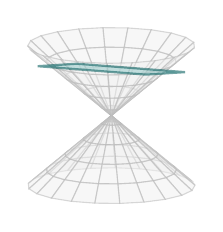
\begin{tikzpicture}
\begin{axis}[hide axis, view={110}{12}, width=4.3cm, height=4.3cm]
\addplot3[surf, shader=faceted, faceted color=gray!55, fill=gray!12, opacity=0.55,
  domain=-1.6:1.6, domain y=0:360, samples=10, samples y=22, z buffer=sort]
  ({x*cos(y)}, {x*sin(y)}, {1.7*x});
\draw[fill=teal!40, opacity=0.55, draw=teal!70!black, thick]
  (axis cs:-1.1,-1.1,1.4) -- (axis cs:1.1,-1.1,2.2) --
  (axis cs:1.1,1.1,2.2) -- (axis cs:-1.1,1.1,1.4) -- cycle;
\end{axis}
\end{tikzpicture}
% 패널 2: 포물선 (모선과 평행한 평면)
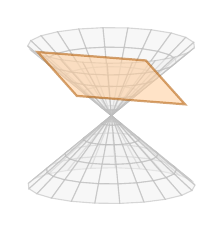
\begin{tikzpicture}
\begin{axis}[hide axis, view={110}{12}, width=4.3cm, height=4.3cm]
\addplot3[surf, shader=faceted, faceted color=gray!55, fill=gray!12, opacity=0.55,
  domain=-1.6:1.6, domain y=0:360, samples=10, samples y=22, z buffer=sort]
  ({x*cos(y)}, {x*sin(y)}, {1.7*x});
\draw[fill=orange!40, opacity=0.55, draw=orange!70!black, thick]
  (axis cs:-1.1,-1.1,0.15) -- (axis cs:1.1,-1.1,2.75) --
  (axis cs:1.1,1.1,2.75) -- (axis cs:-1.1,1.1,0.15) -- cycle;
\end{axis}
\end{tikzpicture}
% 패널 3: 쌍곡선 (축에 가까운 급한 평면, 양쪽 nappe 통과)
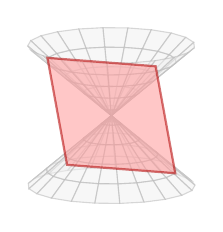
\begin{tikzpicture}
\begin{axis}[hide axis, view={110}{12}, width=4.3cm, height=4.3cm]
\addplot3[surf, shader=faceted, faceted color=gray!55, fill=gray!12, opacity=0.55,
  domain=-1.6:1.6, domain y=0:360, samples=10, samples y=22, z buffer=sort]
  ({x*cos(y)}, {x*sin(y)}, {1.7*x});
\draw[fill=red!40, opacity=0.55, draw=red!70!black, thick]
  (axis cs:-0.55,-1.1,-2.3) -- (axis cs:0.55,-1.1,2.3) --
  (axis cs:0.55,1.1,2.3) -- (axis cs:-0.55,1.1,-2.3) -- cycle;
\end{axis}
\end{tikzpicture}
\caption{직원추면(회색)을 각기 다른 각도의 평면(색 있는 사각형)으로 자를 때: 왼쪽부터 타원, 포물선, 쌍곡선 단면}
\end{figure}

이 정리에 의해 이차곡선을 \textbf{원추곡선}(conic section)이라고도 한다.

\subsection*{EXAMPLE 4}
\(4x^2-3y^2+12z^2-16x-30y-24z-47=0\)이 표시하는 곡면은?\\
\textbf{SOLUTION:} 완전제곱꼴로 정리하면
\[
4(x-2)^2-3(y+5)^2+12(z-1)^2=0
\quad\Longrightarrow\quad
\frac{(x-2)^2}{3}-\frac{(y+5)^2}{4}+(z-1)^2=0
\]
정점 \((2,-5,1)\), 축이 \(zx\)평면에 수직인 \textbf{타원추면}.

\section*{[4] 회전면 (Surface of Revolution)}

\begin{tcolorbox}[
    colback=teal!4,
    colframe=teal!65!black,
    title=정의 \& 핵심 규칙,
    fonttitle=\bfseries,
    boxrule=0.5mm,
    arc=3mm
    ]
    \textbf{\textcolor{teal!65!black}{정의.}}\quad
    평면곡선을 한 직선(회전축)에 대해 회전시켜 만든 곡면이 \textbf{회전면}이다.

    \noindent\textcolor{teal!50!black}{\rule{\linewidth}{0.4pt}}

    \textbf{\textcolor{teal!65!black}{핵심 규칙.}}\quad
    회전축이 아닌 변수를 \(\sqrt{(\cdot)^2+(\cdot)^2}\)로 치환한다.
\end{tcolorbox}

\begin{figure}[h]
\centering
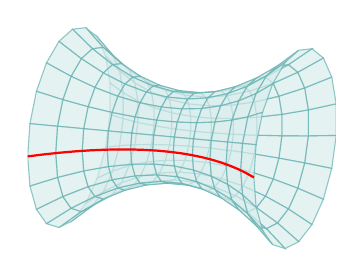
\begin{tikzpicture}
\begin{axis}[hide axis, view={110}{15}, width=5.5cm, height=5.5cm]
\addplot3[
    surf, shader=faceted, faceted color=teal!60, fill=teal!15, opacity=0.7,
    domain=-1.3:1.3, domain y=0:360, samples=12, samples y=20, z buffer=sort,
]
({(0.35*x^2+0.5)*cos(y)}, {x}, {(0.35*x^2+0.5)*sin(y)});
\addplot3[thick, red, domain=-1.3:1.3, samples=20, samples y=0]
({0.35*x^2+0.5}, {x}, {0});
\end{axis}
\end{tikzpicture}
\caption{곡선 $f(x,y)=0$(빨간선)을 $y$축으로 회전시킨 회전면}
\end{figure}

% ---- 그림 삽입 위치 3: 회전면 생성 원리 ----

\begin{center}
\renewcommand{\arraystretch}{1.3}
\begin{tabular}{|l|l|}
\hline
원래 곡선 & 회전축 $\to$ 회전면의 방정식 \\
\hline
\(xy\)평면, \(f(x,y)=0\) & \(y\)축: \(f(\sqrt{x^2+z^2},y)=0\) \\
\hline
\(xy\)평면, \(f(x,y)=0\) & \(x\)축: \(f(x,\sqrt{y^2+z^2})=0\) \\
\hline
\(yz\)평면, \(f(y,z)=0\) & \(y\)축: \(f(y,\sqrt{x^2+z^2})=0\) \\
\hline
\(yz\)평면, \(f(y,z)=0\) & \(z\)축: \(f(\sqrt{x^2+y^2},z)=0\) \\
\hline
\(zx\)평면, \(f(z,x)=0\) & \(z\)축: \(f(z,\sqrt{x^2+y^2})=0\) \\
\hline
\(zx\)평면, \(f(z,x)=0\) & \(x\)축: \(f(\sqrt{y^2+z^2},x)=0\) \\
\hline
\end{tabular}
\end{center}

\subsection*{EXAMPLE 5}
직선 \(z=mx\)를 \(x\)축에 대해 회전시킨 직원 추의 방정식을 구하여라
\textbf{SOLUTION:} $\to$ \(z\) 대신 \(\sqrt{y^2+z^2}\) 대입:
\[
y^2+z^2=m^2x^2 \quad(\text{직원추면})
\]
\subsection*{EXAMPLE 6}
원 \((x-a)^2+z^2=b^2,\ y=0\)을 \(z\)축에 대해 회전시킨 원환면의 방정식을 구하여라
\textbf{SOLUTION:} $\to$ \(x\) 대신 \(\sqrt{x^2+y^2}\) 대입:
\[
\left(\sqrt{x^2+y^2}-a\right)^2+z^2=b^2
\ \Longrightarrow\
(x^2+y^2+z^2+a^2-b^2)^2=4a^2(x^2+y^2)
\]

\begin{figure}[h]
\centering
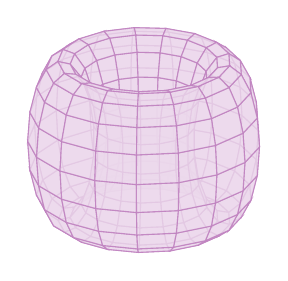
\begin{tikzpicture}
\begin{axis}[hide axis, view={115}{25}, width=5.5cm, height=5.5cm]
\addplot3[
    surf, shader=faceted, faceted color=violet!50, fill=violet!15, opacity=0.8,
    domain=0:360, domain y=0:360, samples=18, samples y=18, z buffer=sort,
]
({(2+0.8*cos(y))*cos(x)}, {(2+0.8*cos(y))*sin(x)}, {0.8*sin(y)});
\end{axis}
\end{tikzpicture}
\caption{원환면(torus)}
\end{figure}
% ---- 그림 삽입 위치 4: 완성된 원환면 ----
\section*{연습문제 7.1}
\begin{enumerate}
    \item 점 \(A(1,0,0),\ B(0,2,0),\ C(0,0,3),\ O(0,0,0)\)을 지나는 구면의 방정식을 구하여라.
    \item 점 \((1,2,3)\)을 중심으로 하고 \(yz\)평면에 접하는 구면의 방정식을 구하여라.
    \item 다음 추면의 방정식을 구하여라.
    \begin{enumerate}
        \item[(1)] 원점을 정점, 원 \(x=a,\ y^2+z^2=b^2\)을 도선
        \item[(2)] 원점을 정점, \(y^2=-2z+4,\ x=3\)을 도선
    \end{enumerate}
    \item 다음 주면의 그래프를 그려라.
    \begin{enumerate}
        \item[(1)] \(x^2-y^2=1\)
        \item[(2)] \(y^2=4x\)
    \end{enumerate}
\end{enumerate}
\end{document}
